\documentclass{report}
\usepackage{titlesec}
\usepackage {mcode} 					% matlab formatting
\usepackage{graphicx}
\DeclareGraphicsExtensions{.jpg, .png}
\titleformat{\chapter}
  {\normalfont\LARGE\bfseries}{\thechapter}{1em}{}
\titlespacing*{\chapter}{0pt}{3.5ex plus 1ex minus .2ex}{2.3ex plus .2ex}
\parindent0pt  \parskip10pt             % make block paragraphs
\raggedright                            % do not right-justify

\title{\bf Introduction to Vision and Robotics Assessed Practical 1: Robot Tracking}  % Supply information
\author{
	Ran Guan\\
	\and
	Thea Koutsoukis\\            
}
\date{4pm March 7, 2013}                           

\begin{document}                        % End of preamble, start of text.
\maketitle                              % Print title page.
\pagenumbering{roman}                   % roman page number for toc
\setcounter{page}{2}                    % make it start with "ii"
\tableofcontents         
\renewcommand{\chaptername}{}           % Print table of contents

\chapter{Introduction}                	% Print a "chapter" heading
\pagenumbering{arabic}                  % Start text with arabic 1
Our strategy for this task was to smooth the image, normalise the colors to account for the difference in illumination, set a threshold for the our definition of red, green and blue and then focus on a small section of the robot to get direction and trajectory
 
\chapter{Methods}                		
\section{Smoothing}                  	

We smoothed the image to remove noise in the image using two built-in matlab methods, fspecial and imfilter. In detectSingleImage, we used fspecial to create a circular averaging filter with a radius of 10. In deciding whether to use the circular or gaussian filter, two factors came into play. First, the robots we are trying to detect are so distinct from the background, and the nature of the scene is so artificial that the distribution of color pixels is closer to a step function than a gaussian function. This meant the circular filter could perform just as well as the gaussian but potentially faster. Secondly, the circular filter takes less arguments (just a radius size, as opposed to the filter size and sigma arguments needed by gaussian), meaning that experimenting with different values was easier. The radius was found by trial and error, a smaller radius did produce a clearer robot, but caused problems with strings and shadows still being too visible. imfilter then applied this circular filter to the image.

Smoothing with radius 5 and 10:

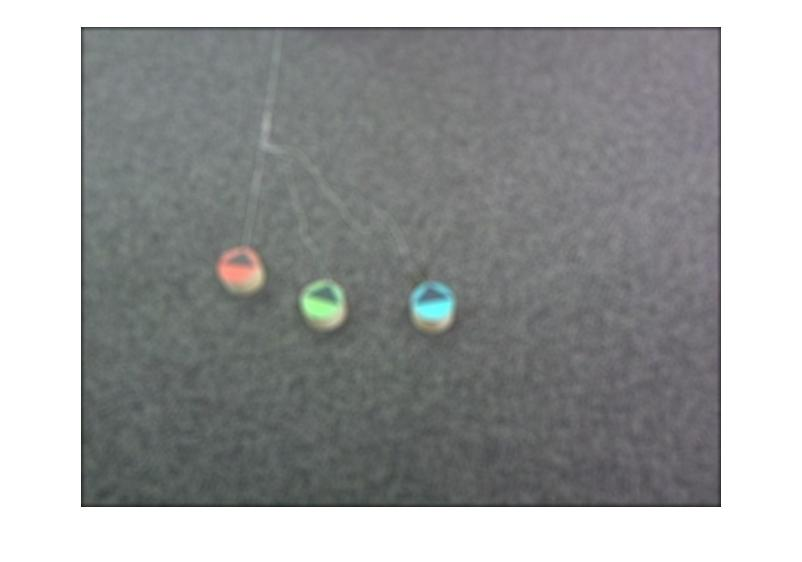
\includegraphics[scale=0.2]{radius5}
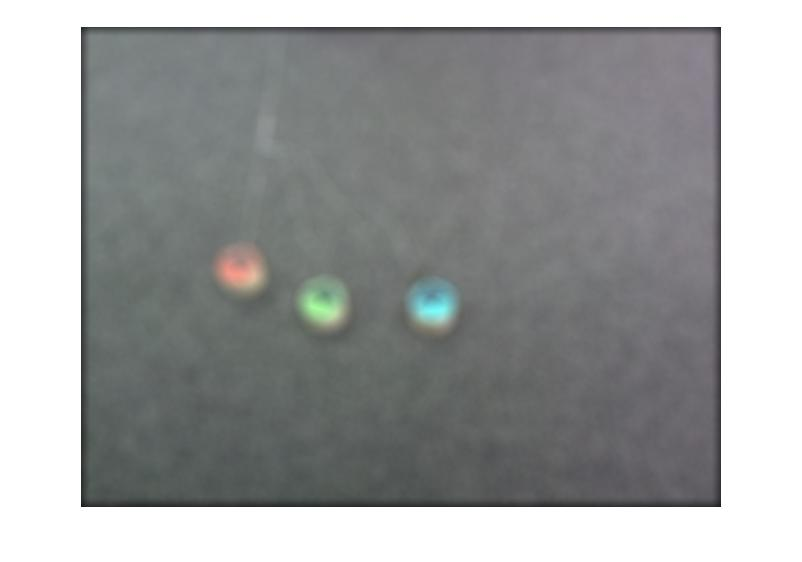
\includegraphics[scale=0.2]{radius10} 

\section{Normalisation}
             
To cope with varying lighting, we normalised the image through the function normaliseColor. This takes an image and brightens it up, using the formula for RGB normalisation given in the lectures. A value too small produced a completely black image, whilst a too large value caused the image to be overexposed. Experimentation proved 500 to be the optimal value. 

\section{Robot Detection}
First of all, we approximated a background image. This involved finding the average rgb value for the background using meanBG, by summing up the rgb value of each pixel and dividing by the number of pixels. Then we examined each pixel of the image. If the color value of this pixel was close to the mean, we set it as the background. Otherwise it was set to being part of the foreground. The "distance", or similarity of one color to another was computed using our colorSimilarity function. This is a normalised euclidean distance, as each color behaves differently. A small distance between the r values for a particular pixel means more than the same distance between b values, so dividing by a different constant for each returns a more accurate similarity.
The foreground image was then passed through the function labelRegion. The image was converted to black and white, and if the black region was large enough it was determined to be a robot. To label each specific color, a pixel in the original image was examined and the highest color channel determined the color of the robot.

\section{Direction}
The direction of the robot was found by isolating a small section in the middle of the robot and drawing a straight line from the centre to the midpoint of the black. In most cases, this was accurate enough to correctly determine the direction, however we occasionally ran into trouble when not enough of the black was picked up. This meant the line wasn't being drawn to the tip of the arrow, but to somewhere in the middle. 

Region of Interest and Computed Direction: (note how not enough black was picked up on the red robot, thus the direction is slightly off)

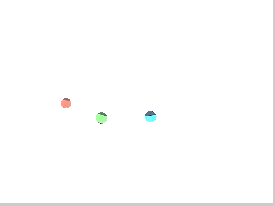
\includegraphics[scale=0.7]{regionofinterest}
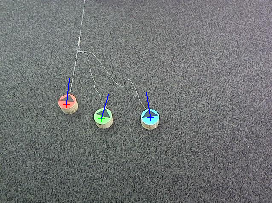
\includegraphics[scale=0.7]{direction}


\chapter{Results}   

\section{Dataset 1}
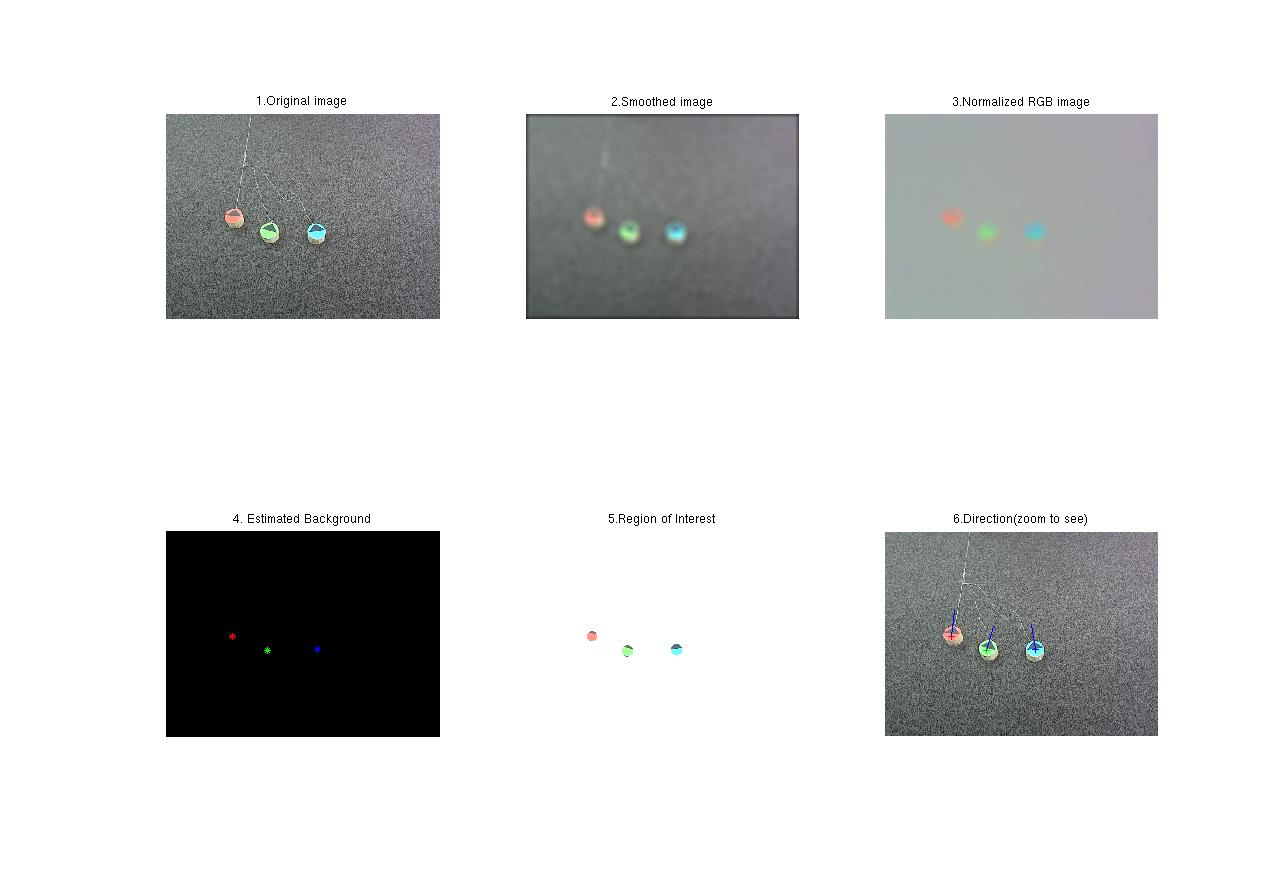
\includegraphics[scale=0.3]{example}

\section{Dataset 2}
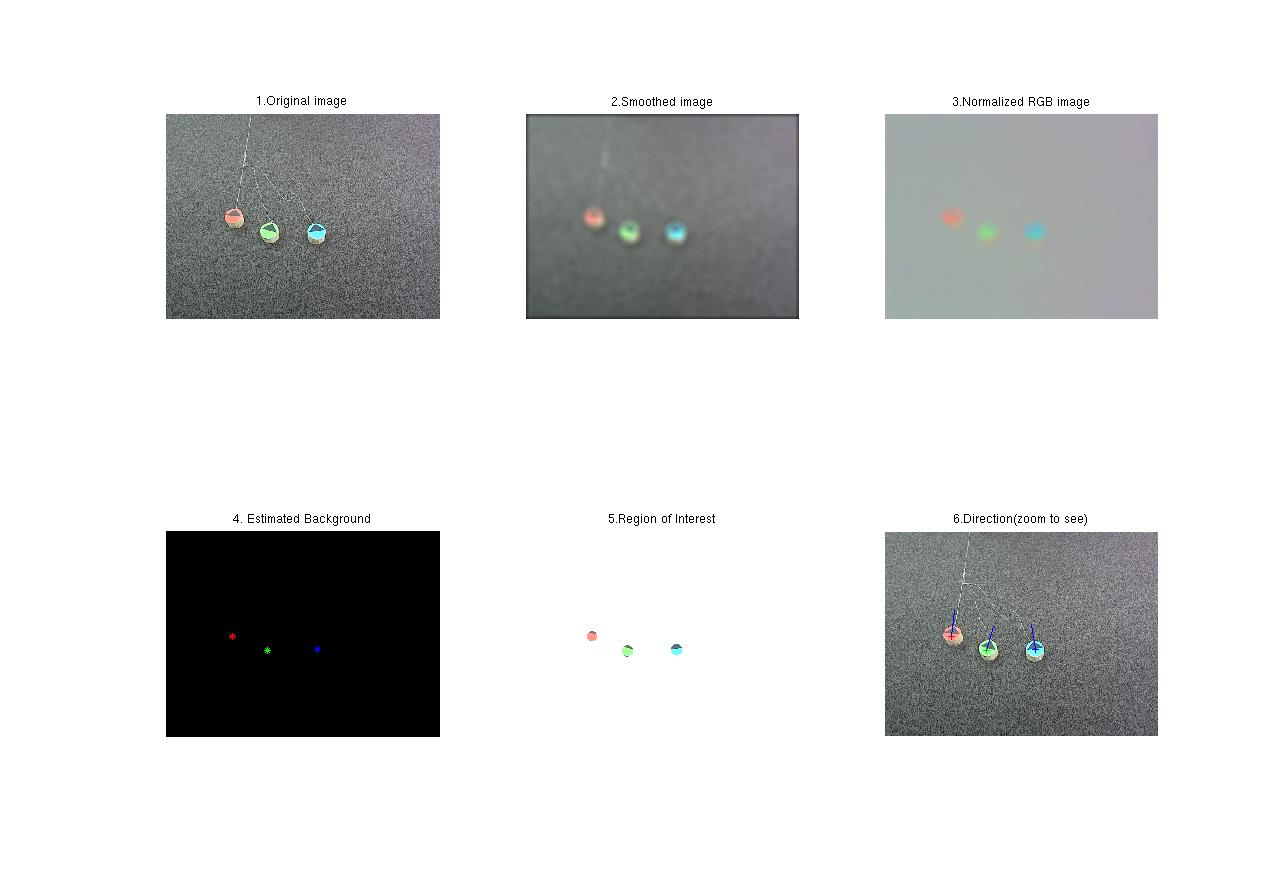
\includegraphics[scale=0.3]{example}

\section{Own Data}
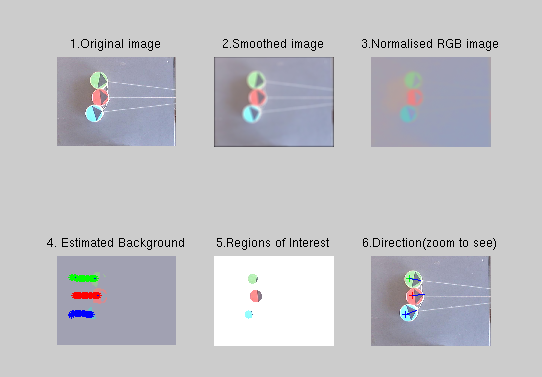
\includegraphics[scale=0.3]{data3}
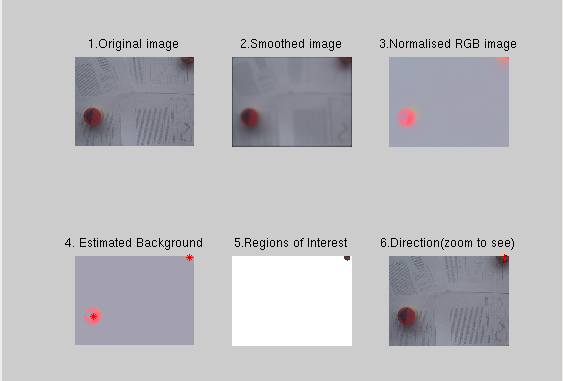
\includegraphics[scale=0.3]{datasetred}
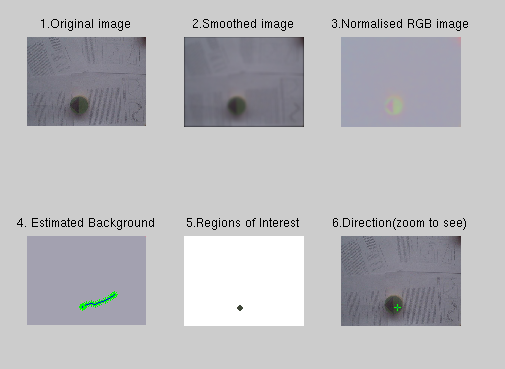
\includegraphics[scale=0.3]{datasetgreen}

Our program worked surprisingly well for our own datasets. A few interesting examples are included here.
In the datasets with more than one robot of each color, our program did not succeed for red, but did for green and blue. 

\chapter{Discussion}            

Our program is successful once we fine tune the constants for each particular data set. Unfortunately, we couldn't get adaptive thresholding to accurately work any better than just using the constants that had been set for another set of images. Thus, if our program was tried out on different sized robots, it would likely not perform very well. We would have liked to improve the estimated background image. At the moment, it's only a crude approximation, and only works well on uniform backgrounds. Large shadows and variations in texture and lighting don't show up, so there is definitely room for improvement there. 

\chapter{Code}
euclidianDist2D
\lstinputlisting{/afs/inf.ed.ac.uk/user/s10/s1009894/Desktop/ThirdYear/Semester2/IVR/Assignment1/ivr-practical1/Code/euclideanDist2D.m} % Inserts code from this file
colorSimilarity
\lstinputlisting{/afs/inf.ed.ac.uk/user/s10/s1009894/Desktop/ThirdYear/Semester2/IVR/Assignment1/ivr-practical1/Code/colorSimilarity.m}
labelRegion
\lstinputlisting{/afs/inf.ed.ac.uk/user/s10/s1009894/Desktop/ThirdYear/Semester2/IVR/Assignment1/ivr-practical1/Code/labelRegion.m}
normaliseColor
\lstinputlisting{/afs/inf.ed.ac.uk/user/s10/s1009894/Desktop/ThirdYear/Semester2/IVR/Assignment1/ivr-practical1/Code/normaliseColor.m}
meanBG
\lstinputlisting{/afs/inf.ed.ac.uk/user/s10/s1009894/Desktop/ThirdYear/Semester2/IVR/Assignment1/ivr-practical1/Code/meanBG.m}
diffFromBG
\lstinputlisting{/afs/inf.ed.ac.uk/user/s10/s1009894/Desktop/ThirdYear/Semester2/IVR/Assignment1/ivr-practical1/Code/diffFromBG.m}
segmentFromRadius
\lstinputlisting{/afs/inf.ed.ac.uk/user/s10/s1009894/Desktop/ThirdYear/Semester2/IVR/Assignment1/ivr-practical1/Code/segmentFromRadius.m}
detectSingleImage
\lstinputlisting{/afs/inf.ed.ac.uk/user/s10/s1009894/Desktop/ThirdYear/Semester2/IVR/Assignment1/ivr-practical1/Code/detectSingleImage.m}
trackAllImages
\lstinputlisting{/afs/inf.ed.ac.uk/user/s10/s1009894/Desktop/ThirdYear/Semester2/IVR/Assignment1/ivr-practical1/Code/trackAllImages.m}

link to experimental datasets: https://github.com/theakaterina/ivr-practical1

\chapter{Note on Mark Distribution}
Ran did the majority of the coding within the first week of the assignment being released. The next two weeks Thea spent cleaning up code, adjusting constants and writing the report. We propose the marks be split 60:40 in Ran's favour.

\end{document}                       % The required last line
